\section{Client Usage}
\label{sec:client_usage}
The \aclient[] can generally do three things; commit a problem, see status of his/her problems, or search the database for problems.
The first two are based on their corresponding use cases in section \ref{sec:usecase}.
The search function was added as a functionality for \aclient[] because we assume that it would primarily be persons with a new problem who might want to search for others problems.

The following subsections describes the three usage of the application which the \aclient[] has access to.
The process of searching for problems and seeing status of the \aclient[]s problems have switch places in the subsections below because in order for a \aclient[] to check the status of his/her problems a search will be initiated.

\subsection{Commit a Problem}
\label{sub:commit}
The process of committing a problem consists of three steps: Categorizing the problem, considering existing problems, and if no problems suffice the to match the new problem; a creation step.

\subsubsection{Categorizing the Problem}
\begin{figure}[htb]
	\centering
		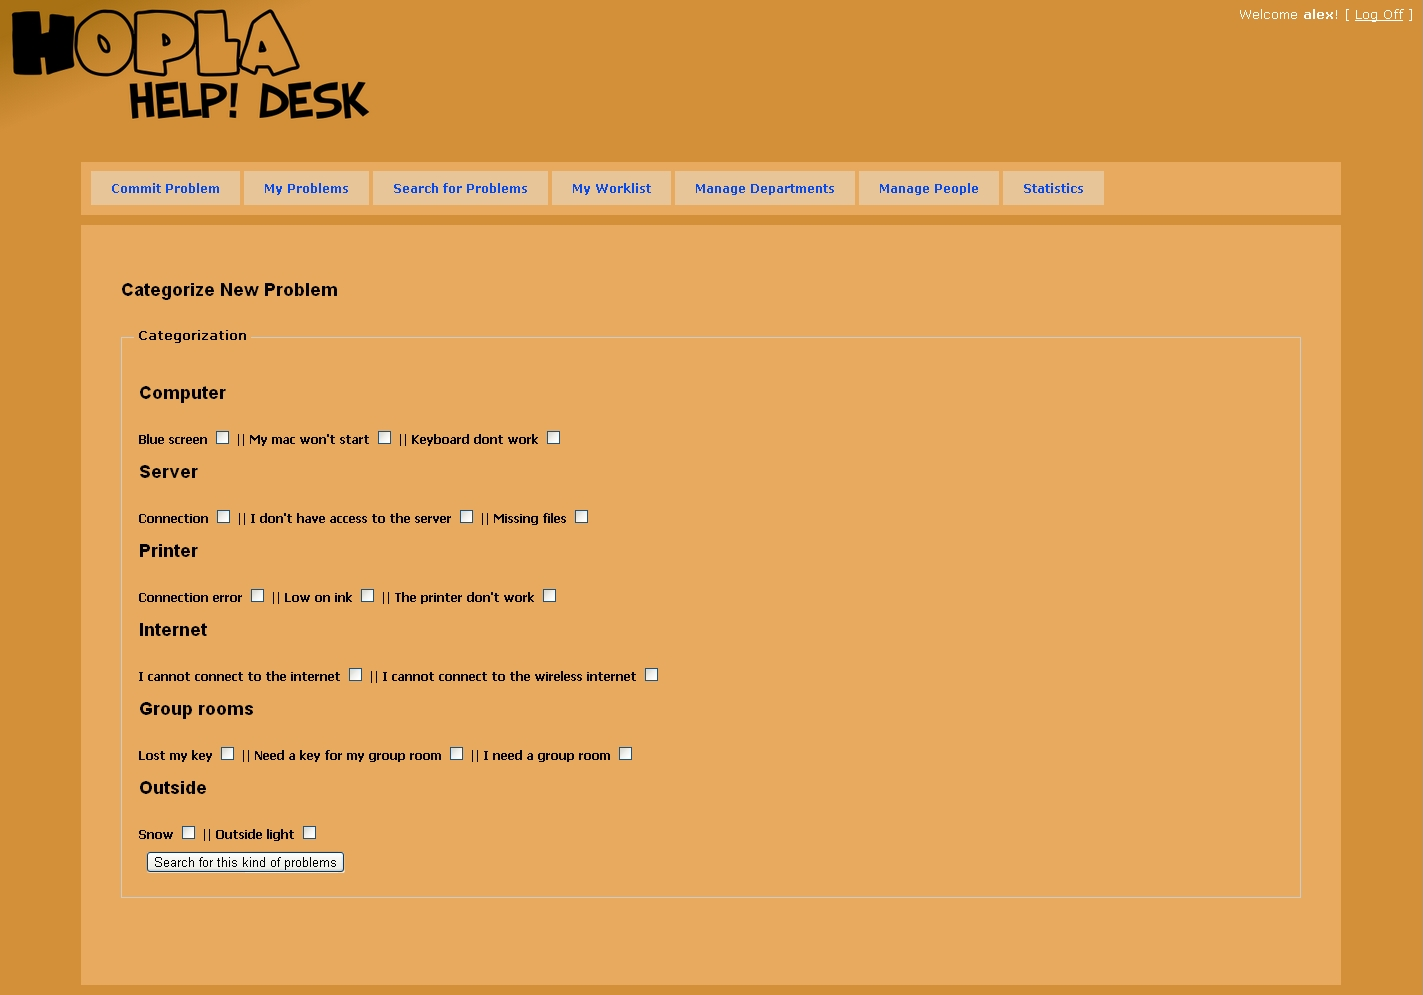
\includegraphics[width=1.00\textwidth, clip=true, trim=2.9cm 0.5cm 15cm 8cm]{input/implementation/program_presentation/commit.png}
	\morscaption{The categorization step in committing a problem, note that the page has been cropped}
	\label{fig:commit}
\end{figure}
The process of committing a problem starts with a click on the Commit Problem menu point, which can be seen in figure \ref{fig:master}.
When Commit Problem is clicked the user is asked to categorize the problem in the window showed in figure \ref{fig:commit}.
As the figure shows the tags, the check boxes, are ordered under headlines.
These headlines are categories.

\subsubsection{Consider Existing Problems}
\label{ssu:consider}
When the problem is categorized the application searches for problems matching the specified tags, the search function is described in \ref{sec:search}.
The problems found in the search are listed in a table with columns showing number of matching tags, deadline, estimated time of completion, and title and description.
The last column also shows whether the given problem is solved or not.

\subsubsection{Create New Problem}
\begin{figure}[htb]
	\centering
		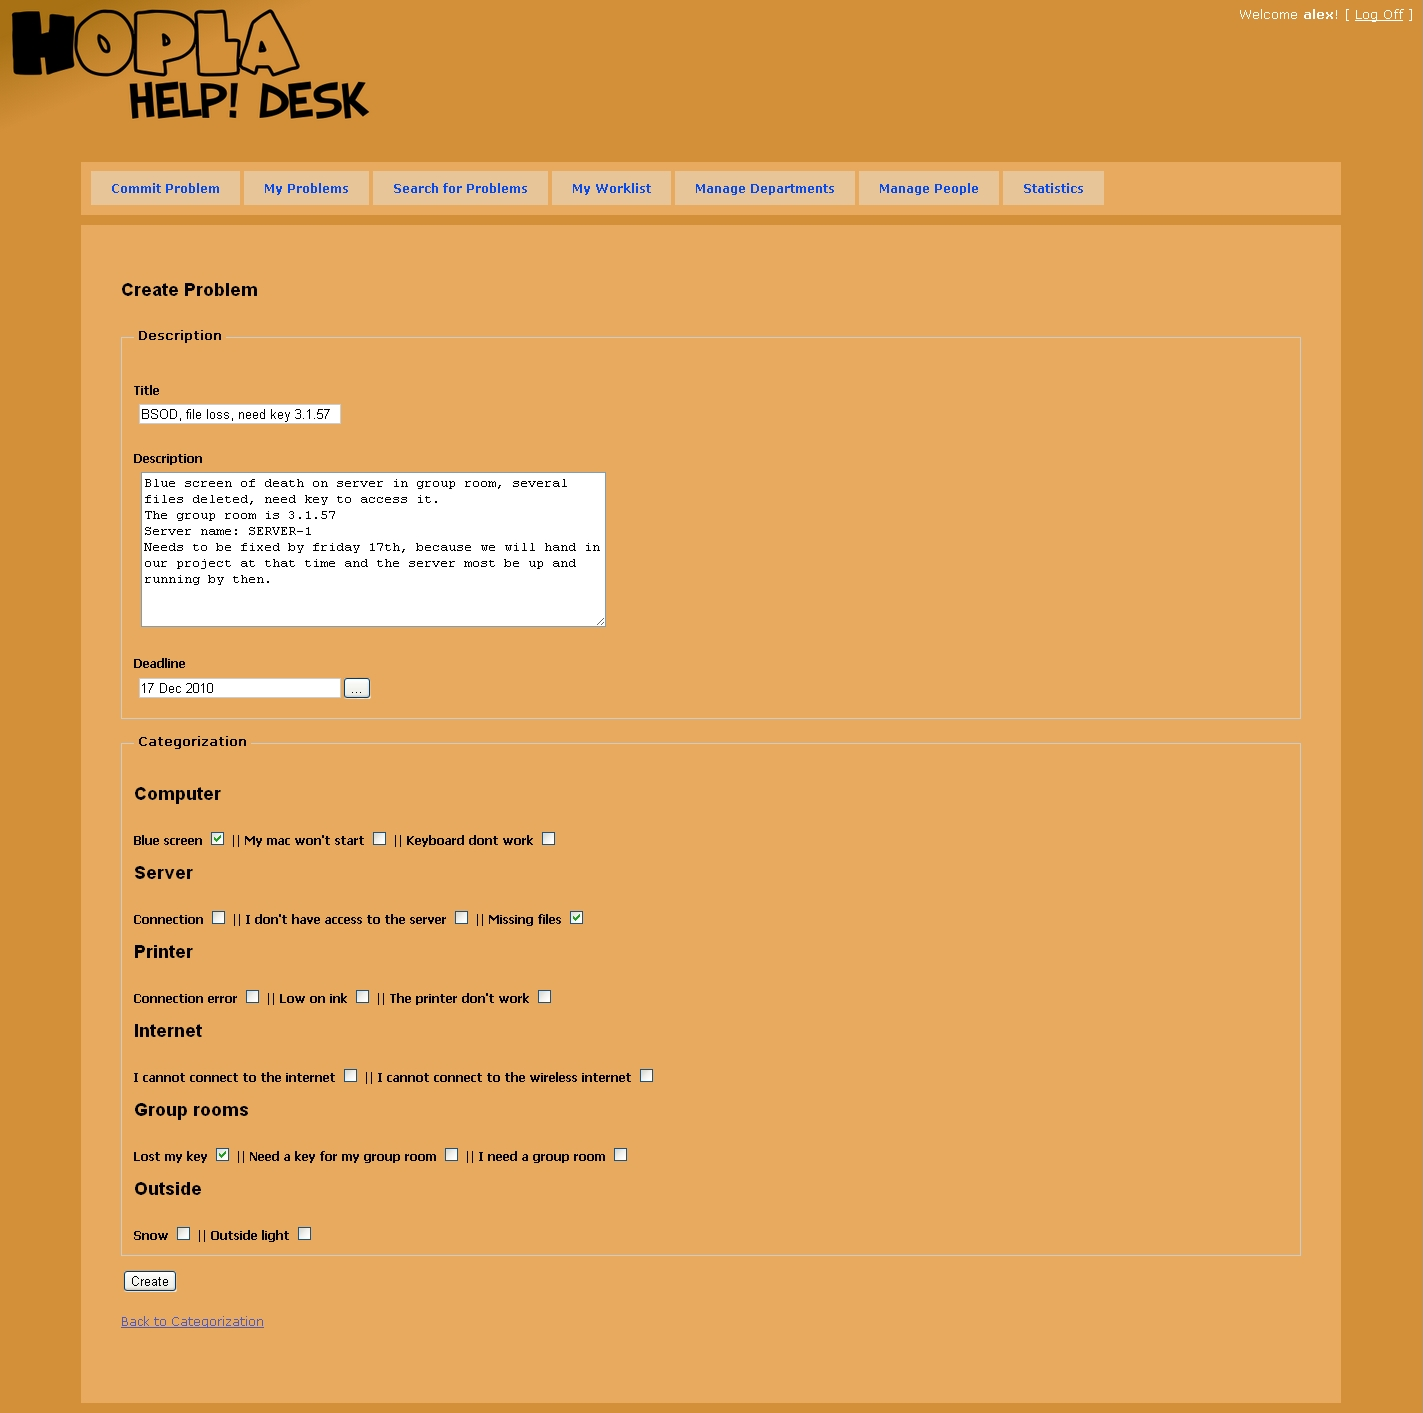
\includegraphics[width=1.00\textwidth, clip=true, trim=2.9cm 0.5cm 15cm 8cm]{input/implementation/program_presentation/newProblem.png}
	\morscaption{The create step of committing a new problem, note that the page has been cropped}
	\label{fig:newProblem}
\end{figure}
The \aclient[] can choose problems and subscribe to them in order to receive notifications when the problems is updated, e.g. a solution is attached to them.
The \aclient[] can also choose to write a new problem if none of the existing problems suffice to match his/her problem.
The screen showed when creating a new problem is seen in figure \ref{fig:newProblem}.
The categorization part of this page remembers what was entered in the categorization step, but allows the \aclient[] to change it if he/she wants to reconsider the chosen tags.
The tags which were marked in the categorization step are remembered and are also marked when this step is started.

When the problem has been described and given a title it can be created.
Optionally the \aclient[] can give the problem a deadline for the \astaff[] member assigned to the problem to consider.
When the problem is created the \aclient[] is presented with a page showing whether or not the problem was successfully added to the application.
To see the problem later, the \aclient[] can either search for it, as described in subsection \ref{sub:searchUsage}, or go to the My Problems menu point, which is described in subsection \ref{sub:myProblem}.

\subsection{Search for Problems}
\label{sub:searchUsage}
To search for problems, the \aclient[] must select the menu point called Search for Problems, which can be seen in figure \ref{fig:master}.
The page which is then shown can be divided into two fields; search field and result field.
The search field is similar to the categorization step of the commit new problem usage, which can be seen in figure \ref{fig:commit} except that a few more options, namely: Only my problems, only unsolved problems, only solved problems, and minimum number of problems to find.
The three first are represented as check boxes and the last is a text field, which accepts a number above 0.

If the only my problems check box is checked, the result will only show problems which the \aclient[] is subscribed to.
The only solved problems and only unsolved problems check boxes does as their names indicate.
If both check boxes are check, no problems will be found of course.

The minimum number of problems is used as an input to the search function, which specifies how many problems should be found before the search function stops running.
The reason for this is that the search is done stepwise, lowering the bound for similarity at each step.
In order to make the search be fast it then need a number which indicates that the size of the result is satisfactory.
The search function is described more thoroughly in section \ref{sec:search}.

The result field displays the problems found by the search function.
This list is initially empty, because the search button must be clicked in run a search.
The way the problems are displayed resembles the table in the \nameref{ssu:consider} step in section \ref{sub:commit} except that it does not have a column with the number of matching tags but instead has a column with the time it was solved -- if the given problem is solved.
The problems in the list can be clicked to enter the details of the given problem, this detail view is described in the following sub-subsection.

\subsubsection{Problem Details}
\begin{figure}[htb]
	\centering
		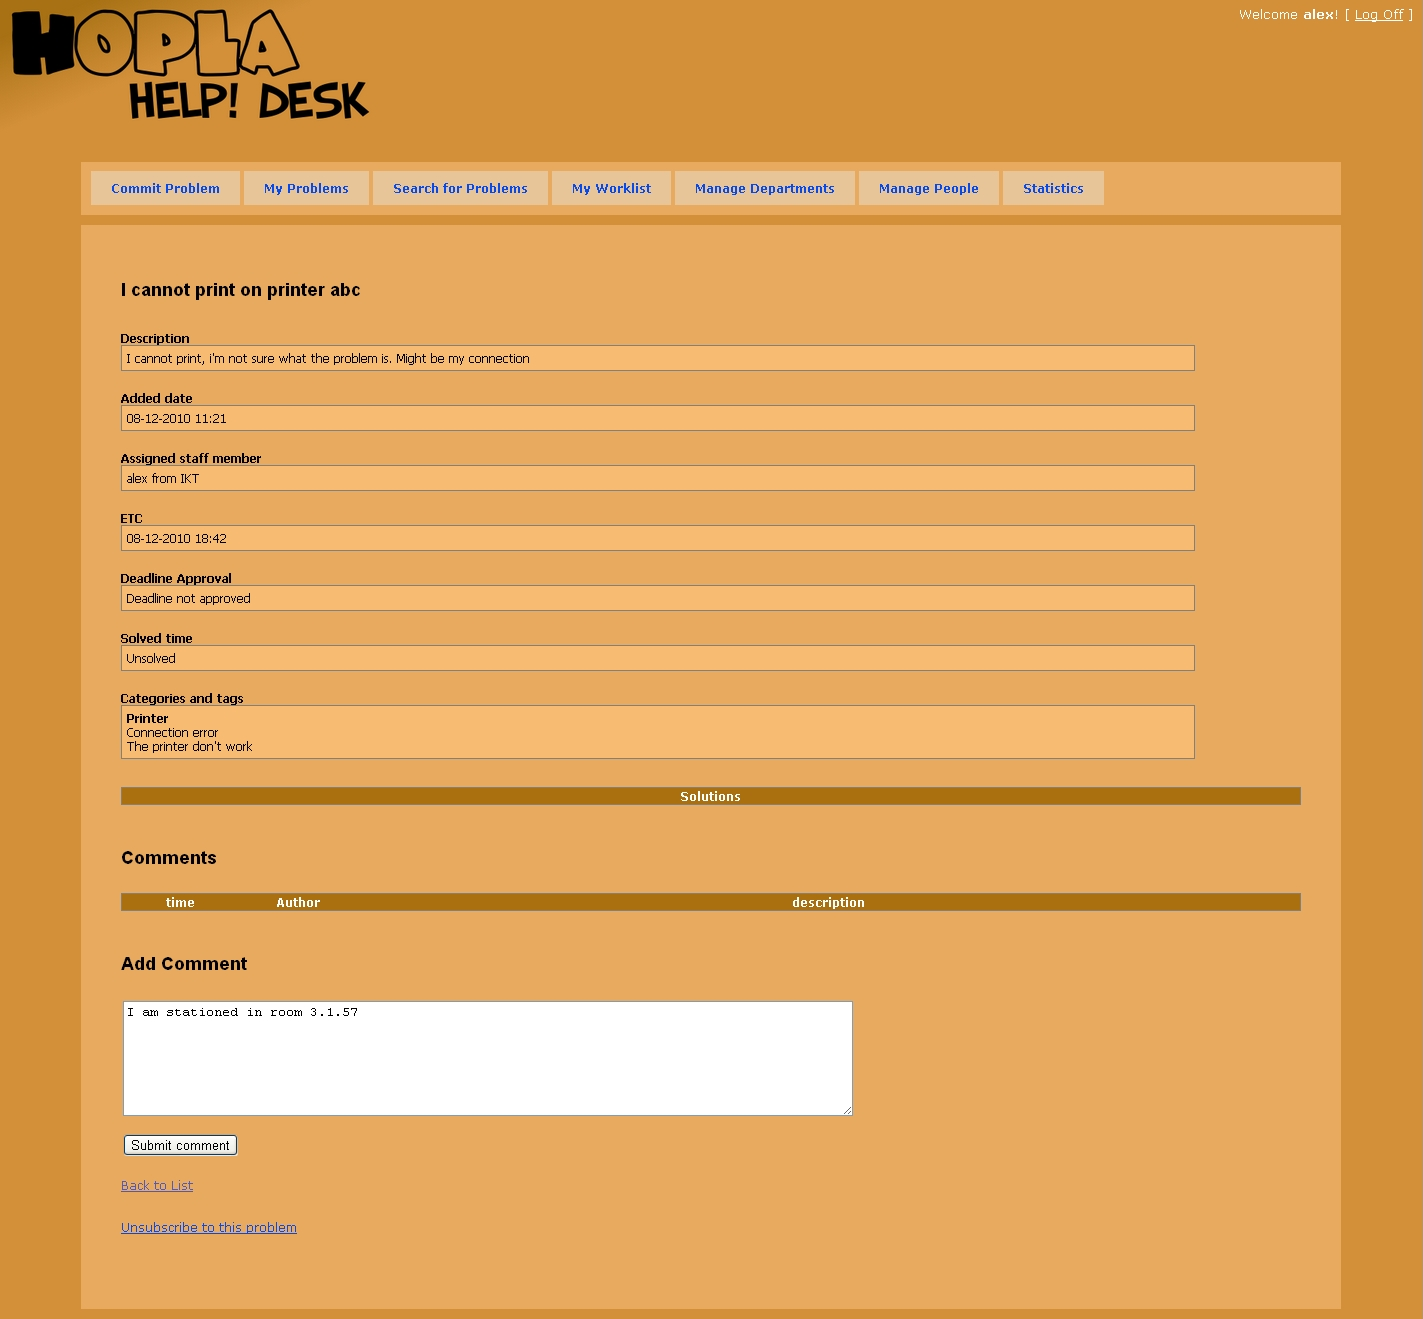
\includegraphics[width=1.00\textwidth, clip=true, trim=2.9cm 0.5cm 3cm 8cm]{input/implementation/program_presentation/problemDetails.png}
	\morscaption{The details of a problem}
	\label{fig:problemDetails}
\end{figure}
The properties of a problem can be seen in the problem details view in figure \ref{fig:problemDetails}.
This view also allows the \aclient[] to add comments to the problem and subscribe or unsubscribe to the problem.
If a \aclient[] is subscribing to a problem, he/she will receive an e-mail every time a solution is added to the problem or when a comment is added.

The details which can be seen in the problem details are: The title, description, added date, assigned to staff member, ETC, deadline approval, solved time, categories and tags, and if the deadline is approved; the actual deadline.
If there is any solutions attached to the problem, these are shown in this view.
The same applies to comments.

\subsection{See Own Problems}
\label{sub:myProblem}
For a \aclient[] to see his/her problems, he/she has the My Problems menu point, which can be seen in figure \ref{fig:master}.
This actually initiates the search for problems process as described in subsection \ref{sub:searchUsage}.
The difference is the headline and the fact that the only my problems and only unsolved problems check boxes are checked.
Also a search is initiated when the menu point is selected.
It is still possible to specify your search further and change the specification of the search, i.e. it works the same way as the search usage described in subsection \ref{sub:searchUsage} from this point on.

